\documentclass[final]{beamer}
\mode<presentation>{\usetheme{MARVEL}}
\usepackage[english]{babel}
\usepackage[latin1]{inputenc}
\usepackage{graphicx}
\usepackage{xcolor}
\usepackage{hyperref}
\usepackage{xparse}
\usepackage{tabularx}
\usepackage{fontawesome5}
\usepackage{listings}
\usepackage[orientation=portrait,size=a0,scale=1.414,debug]{beamerposter}

% setup
\lstset{
  basicstyle=\small\ttfamily,
  columns=fullflexible,
  % frame=single,
  % breaklines=true,
  % postbreak=\mbox{\textcolor{red}{$\hookrightarrow$}\space},
  xleftmargin=2em,
  aboveskip=1em,
  belowskip=1em,
}
\usefonttheme[onlymath]{serif}
%\setbeamertemplate{caption}[numbered]
\graphicspath{{figures/}}
\setbeamertemplate{caption}{\raggedright\insertcaption\par}
\newcounter{blockcounter}
\setcounter{blockcounter}{0}
\newcommand{\nextblocknum}{\stepcounter{blockcounter}\arabic{blockcounter}}
\NewDocumentCommand{\textbox}{ O{\normalsize} O{} m }{\vbox #2{#1{#3}}}
\newcolumntype{L}{X}
\newcolumntype{R}{>{\raggedleft\arraybackslash}X}

% header
\title{ \textbf{\LARGE AiiDA common workflows for computing material properties using different quantum engines} } 
\author{ \textbf{\large \underline{S.P. Huber},$^1$ \textit{et al}} }
\institute{$^1$THEOS and NCCR-MARVEL, \'Ecole Polytechnique F\'ed\'erale de Lausanne (EPFL), Lausanne, Switzerland}

\begin{document}

\begin{frame}[fragile] % note beamer needs fragile for verbatim: https://pbelmans.ncag.info/blog/2011/02/20/why-latex-beamer-needs-fragile-when-using-verbatim/
  %
  \begin{columns}
    %
    %%%%%%%%%%%%%%%%%%%%%%%%%%%%% COLUMN 1 %%%%%%%%%%%%%%%%%%%%%%%%%%%%%%%%%%%%%%%%%%%%
    %
    \begin{column}{.48\textwidth}
      %
      \begin{block}{\centering\textbf{\nextblocknum. Objectives}}
        \textbox{
          The prediction of material properties based on density-functional theory has become routine,
          thanks, in part, to the steady increase in the number and robustness of available simulation packages.
          This diversity of codes and theoretical methods allows scientists the possibility to select the optimal capabilities for their research but,
          conversely, makes it challenging to cross-verify results and combine multiple levels of theory into single workflows.
          We demonstrate how developing common interfaces for workflows that automatically compute material properties greatly simplifies interoperability and cross-verification.
        }
      \end{block}
      %
      \vskip 0.2 cm
      %
      \begin{block}{\centering\textbf{\nextblocknum. Challenges in high-throughput computing}}
        \textbox{
          \noindent
          \begin{itemize}
            \item Workflow automation
                  \begin{itemize}
                    \item Need tools to define complex workflows with advanced error handling
                    \item An automated, robust and scalable engine to run the workflows
                  \end{itemize}
            \item Data management
                  \begin{itemize}
                    \item Data should be stored reliably and efficiently
                    \item Stored data should be interoperable and queryable
                  \end{itemize}
            \item Reproducibility
                  \begin{itemize}
                    \item All produced data should be reproducible by storing the full provenance
                  \end{itemize}
          \end{itemize}
        }
      \end{block}
      %
      \vskip 0.2 cm
      %
      \begin{block}{\centering\textbf{\nextblocknum. AiiDA framework}}
        \textbox{
          The AiiDA framework provides an infrastructure for running complex workflows, automatically tracking each step and organising the full history and results in an easy to query database.
          %
          \vspace{1em}
          %
          \begin{figure}[h]
            \centering
            
\includegraphics[width=0.6\textwidth]{aiida-logo}
          \end{figure}
          %
          \vspace{1em}
          %
          \begin{table}[h]
            \centering
            \begin{tabularx}{0.95\textwidth}{lLRr}
              \large{\faIcon{cog}}\hspace{0.3em}    & \textbf{Scalable workflow engine} & \textbf{Automated data provenance} & \hspace{0.3em}\large{\faIcon{database}} \\
              \large{\faIcon{server}}\hspace{0.3em} & \textbf{Built-in support for HPC} & \textbf{Flexible plugin system}    & \hspace{0.3em}\large{\faIcon{plug}}     \\
              \large{\faIcon{python}}\hspace{0.3em} & \textbf{Python API}               & \textbf{Open Source}               & \hspace{0.3em}\large{\faIcon{osi}}      \\
            \end{tabularx}
          \end{table}
          %
          \vspace{1em}
          %
          \begin{figure}[h]
            \centering
            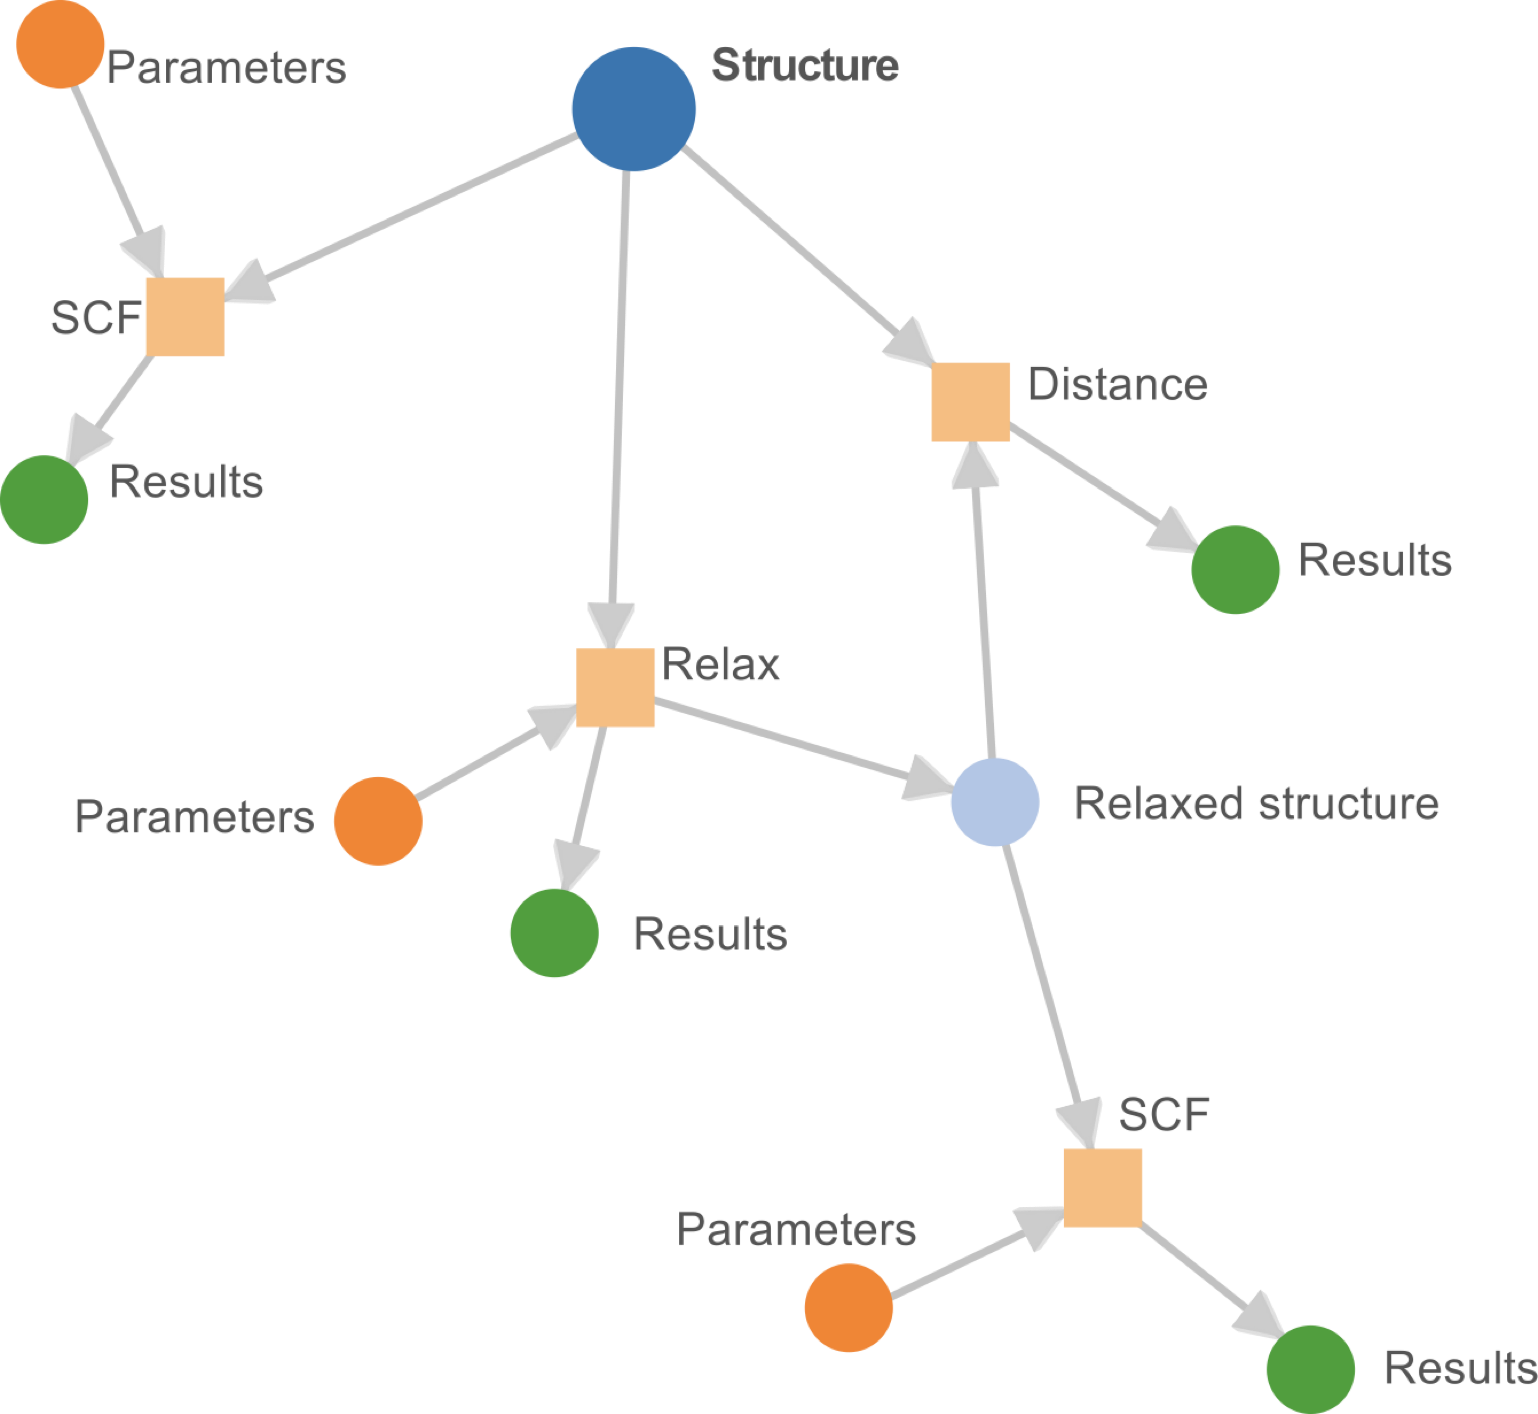
\includegraphics[width=0.55\textwidth]{provenance}
          \end{figure}
        }
      \end{block}
      %
      \vskip 0.2 cm
      %
      \begin{block}{\centering\textbf{\nextblocknum. Common workflow architecture}}
        \textbox{
          \noindent
          \begin{itemize}
            \item Two-stage \textit{opaque transparency} design, to make it both easy for a non-expert to run, and customisable for expert users.
            \item Automatic parameter determination, using protocol ``names''.
            \item Automated handling of failure modes (timeout, convergence, \ldots).
          \end{itemize}
          %
          \vskip 0.2 cm
          %
          \begin{figure}[h]
            \centering
            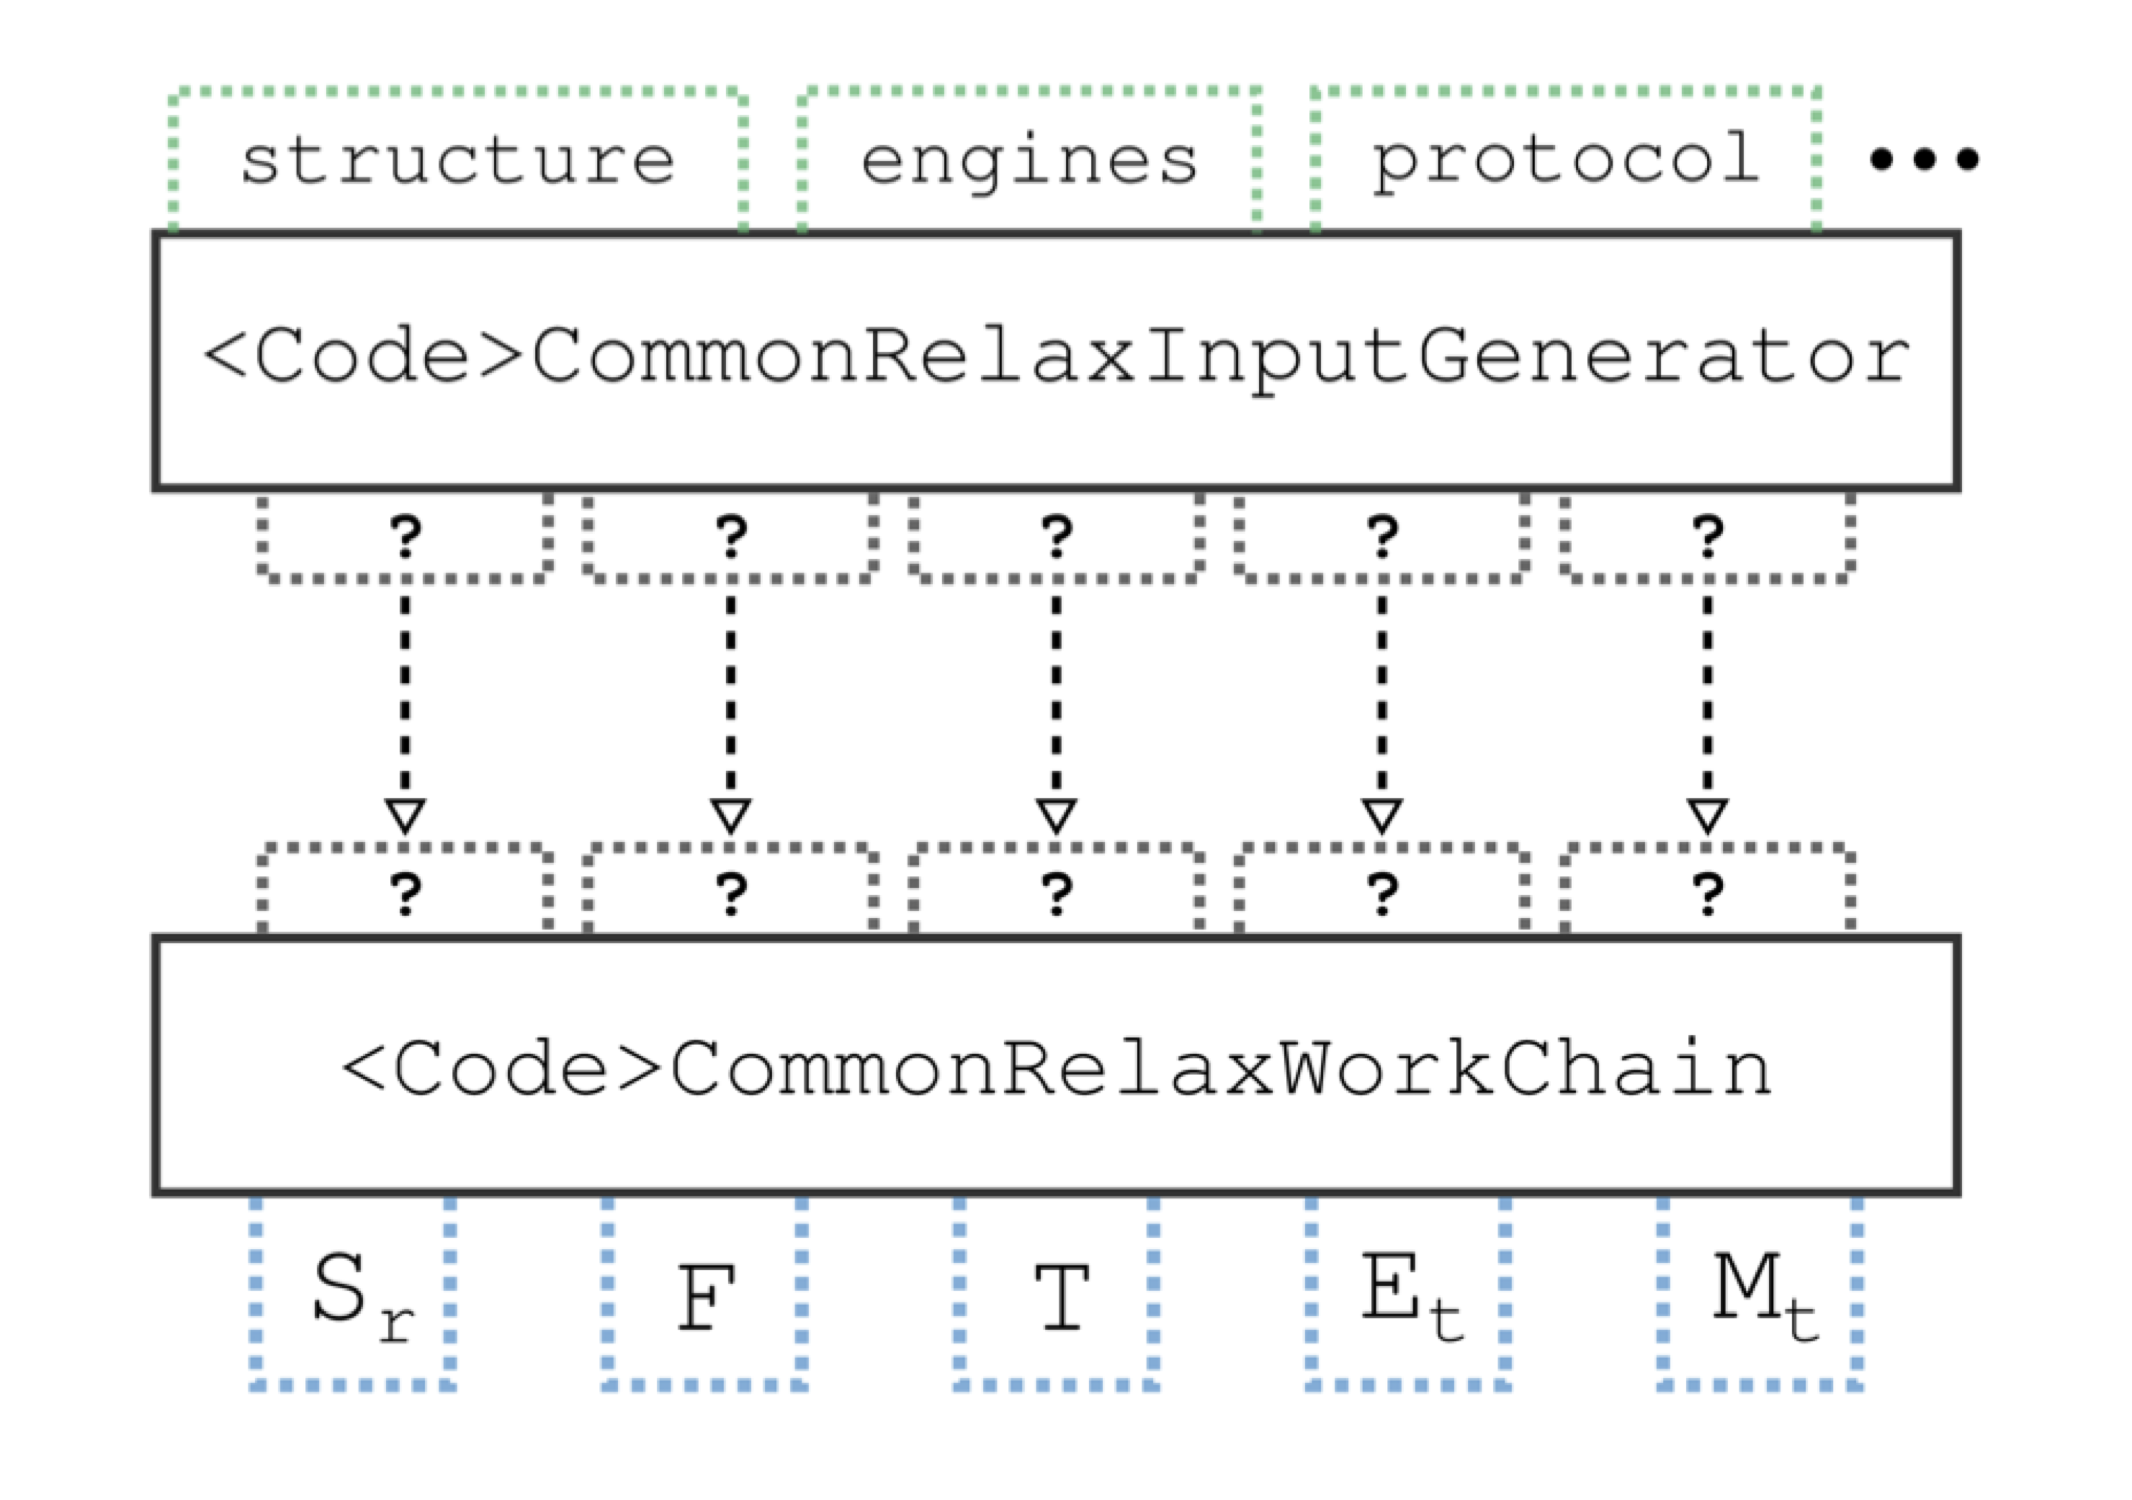
\includegraphics[width=0.6\textwidth]{common-interface}
            \caption{Schematic diagram of the common relax workflow interface.}
          \end{figure}
        }
      \end{block}
    \end{column}
    %
    %%%%%%%%%%%%%%%%%%%%%% COLUMN 2 %%%%%%%%%%%%%%%%%%%%%%%%%%%%%%%%%%%%%%%%%%%%
    %
    \begin{column}{.48\textwidth}
      %
      \begin{block}{\centering\textbf{\nextblocknum. Quantum codes}}
        \textbox{
          The aiida-common-worflows package provides a simple CLI,\textsuperscript{3} for running the workflows, using any of the \textbf{eleven} quantum codes:
        }
        %
        \begin{lstlisting}[language=bash]
$ aiida-common-workflows \
    launch eos siesta --structure=Al --protocol=precise
        \end{lstlisting}
        %
        \begin{figure}[h]
          \centering
          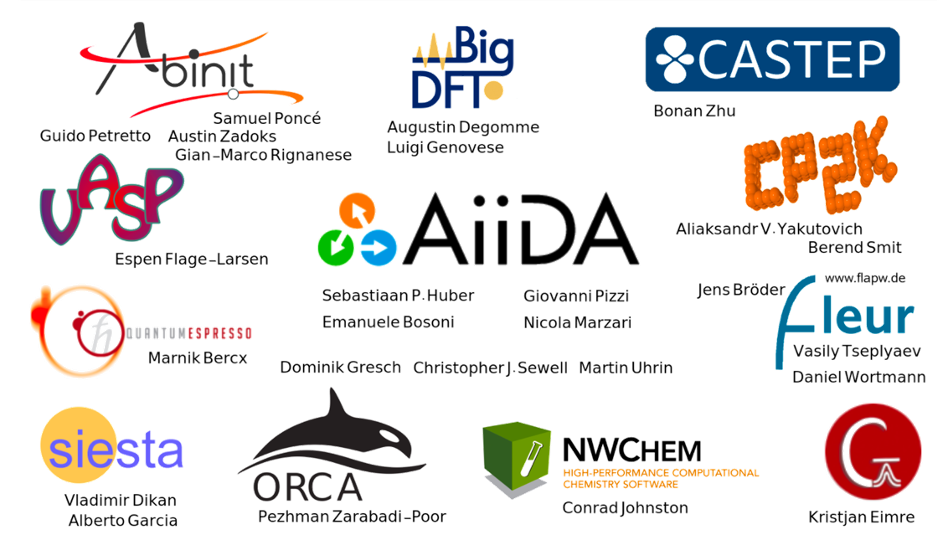
\includegraphics[width=0.98\textwidth]{codes}
        \end{figure}
      \end{block}
      %
      \vskip 0.2 cm
      %
      \begin{block}{\centering\textbf{\nextblocknum. Results}}
        %
        \textbox{
          \noindent
          \begin{itemize}
            \item Simple cases tested for representative atomic systems: insulator (Si), metal (Al), multi-element (GeTe), magnetic (Fe).
            \item Demonstrates good levels of agreement between the results of the different codes.
          \end{itemize}
          %
          \vskip 1 cm
          %
          \begin{figure}[h]
            \centering
            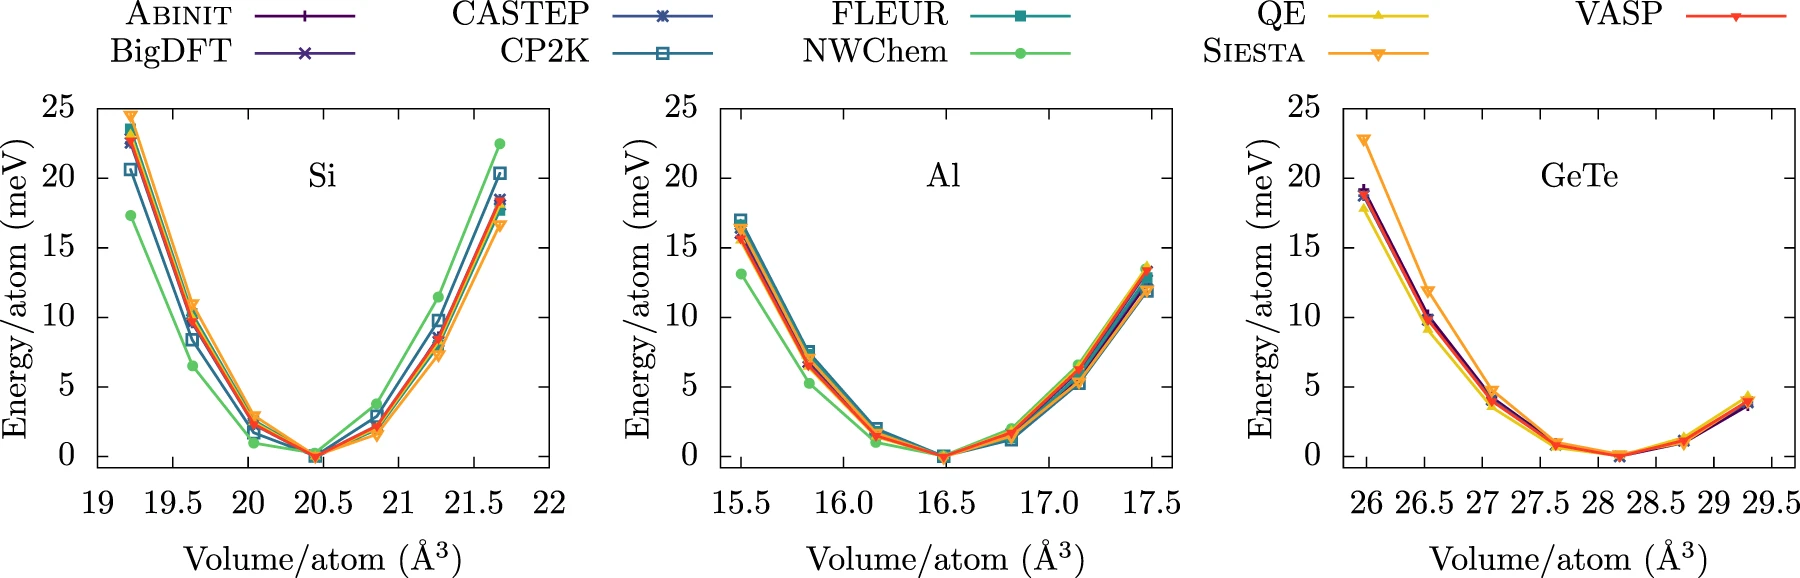
\includegraphics[width=0.9\textwidth]{results_eos1}
            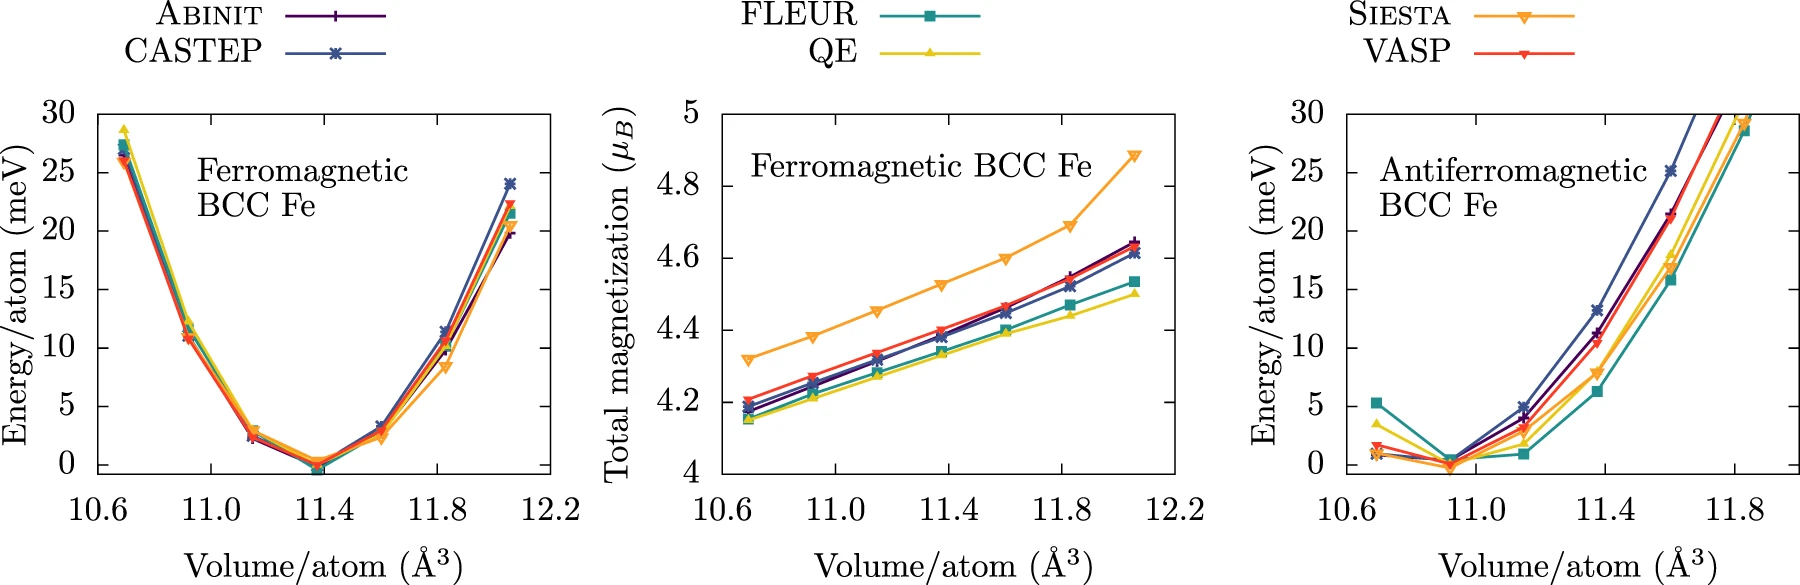
\includegraphics[width=0.9\textwidth]{results_eos2}
            \caption{Results obtained for the Equation of State workflows}
          \end{figure}
          %
          \vskip 0.5 cm
          %
          See Ref. [1] for more details and discussions.
        }
      \end{block}
      %
      %%%%%%%%%%%%%%%%%%%%%%%%%%%%%%%%%%%%%%%%%%%%%%%%%%%%%%%%%%%%%%%%%%%%%%%%%%%%%%%%%
      %
      \vskip 0.2 cm
      %
      \begin{block}{\centering\textbf{\nextblocknum. Summary}}
        %
        \textbox[\normalsize]{
          %
          \begin{itemize}
            \item Open-source, robust turn-key workflows developed for computing materials properties, using the AiiDA framework.
            \item Common interface among 11 quantum engines.
            \item Easy to use, but flexible for experts, designed to be interfaced to GUIs.
            \item Basis of verification studies (oxides set), and starting point for more common workflows.
          \end{itemize}
          %
        }
        %
      \end{block}
      %
      %%%%%%%%%%%%%%%%%%%%%%%%%%%%%%%%%%%%%%%%%%%%%%%%%%%%%%%%%%%%%%%%%%%%%%%%%%%%%%%%%
      %
      \vskip 0.2 cm
      %
      \begin{block}{\centering\textbf{\nextblocknum. References}}
        %
        \textbox[\small]{
          %
          \begin{enumerate}
            \item S.P. Huber \textit{et al}, npj Comput Mater 7, 136 (2021). DOI:~\href{https://doi.org/10.1038/s41524-021-00594-6}{10.1038/s41524-021-00594-6}.
            \item M. Uhrin \textit{et al}, Comp. Mat. Sci., 136 (2021). DOI:~\href{https://doi.org/10.1016/j.commatsci.2020.110086}{10.1016/j.commatsci.2020.110086}.
            \item \href{https://github.com/aiidateam/aiida-common-workflows}{https://github.com/aiidateam/aiida-common-workflows}
            \item \href{https://github.com/aiidateam/aiida-core}{https://github.com/aiidateam/aiida-core}
          \end{enumerate}
          %
        }
        %
      \end{block}
      %
      %%%%%%%%%%%%%%%%%%%%%%%%%%%%%%%%%%%%%%%%%%%%%%%%%%%%%%%%%%%%%%%%%%%%%%%%%%%%%%%%%%%%
      %
      \vskip 0.2 cm
      %
      \begin{block}{\centering\textbf{\nextblocknum. Acknowledgments}}
        %
        \textbox[\small]{
          \parbox{38cm}{This research was supported by the Swiss National Science Foundation (SNSF), through Grant No.~51NF40--182892, and its National Centre of Competence in Research (NCCR) MARVEL, the European H2020 Intersect project through Grant No.~824143~\&~814487.}
        }
        %
      \end{block}
      %
    \end{column}
    %
  \end{columns}
  %
  %%%%%%%%%%%%%%%%%%%%%%%%%%%%%%%%%%%%%%%%%%%%%%%%%%%%%%%%%%%%%%%%%%%%%%%%%%%%%%%%%%%%%%%%
  %
  \begin{columns}
    %
    \begin{column}{.15\textwidth}
      %
      \begin{figure}[h]
        \hspace{-1.5cm}
        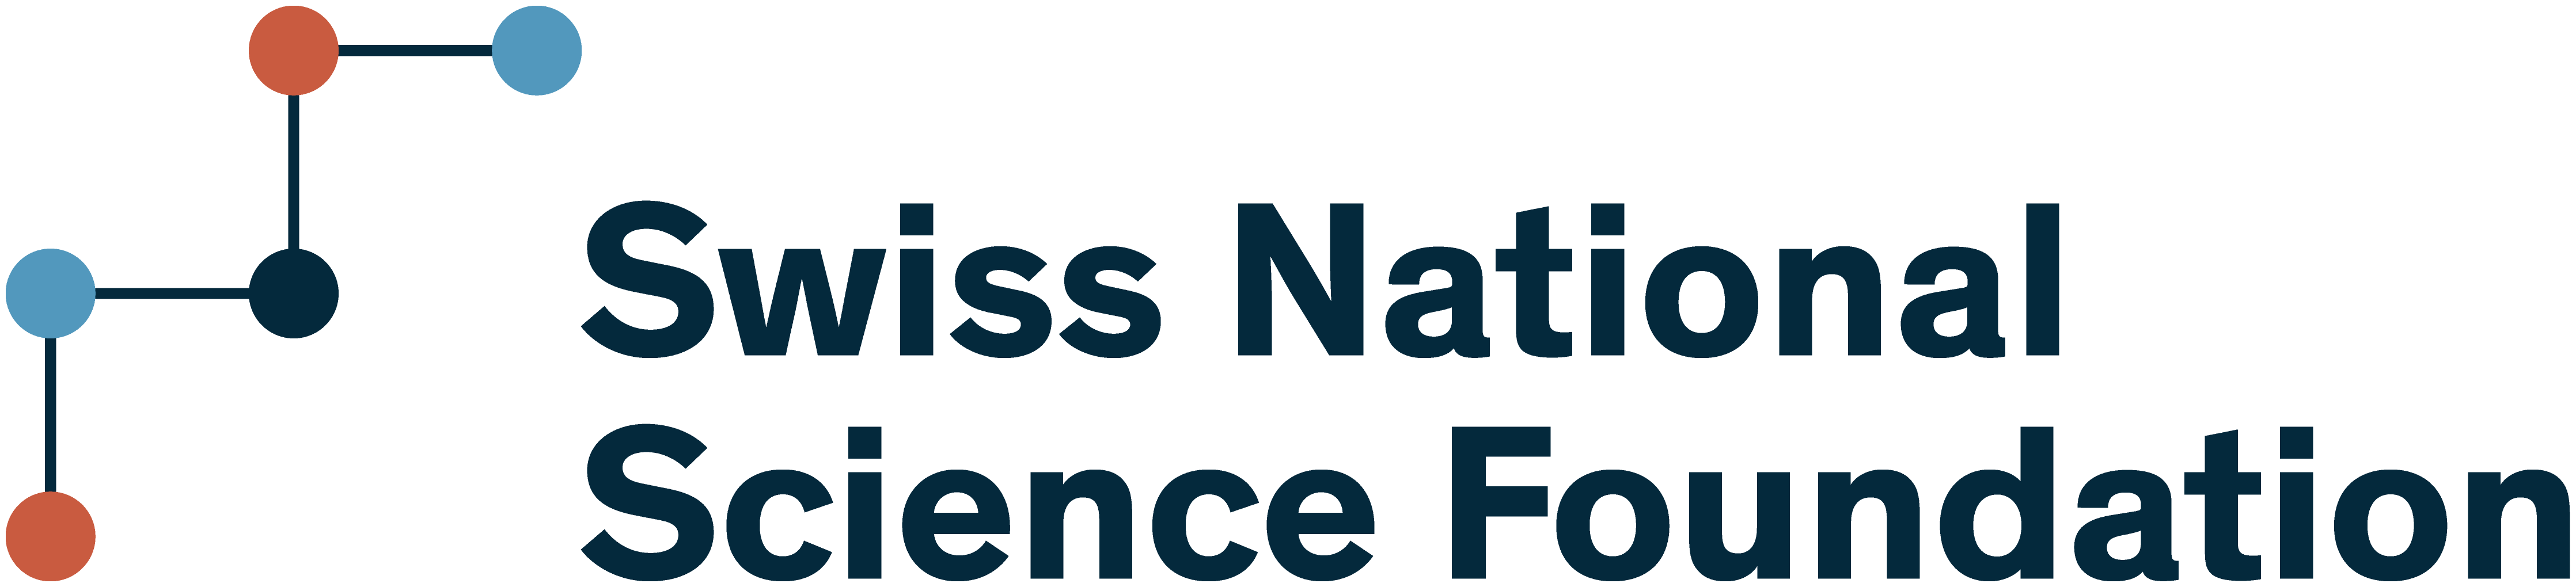
\includegraphics[width=.8\linewidth]{logo_fnsnf}
      \end{figure}
      %
    \end{column}
    %
    \begin{column}{.85\textwidth}
      \vskip 0.1cm
      \hspace{-1.5cm}
      \hbox to 20cm{\small{The National Centres of Competence in Research (NCCR) are a research instrument of the Swiss National Science Foundation}}
    \end{column}
    %
  \end{columns}
  %
  \vfill
  %
\end{frame}

\end{document}
